\chapter{Ошибки и исключения}
\label{errors-and-exceptions}
\section{Придержи коней!}
\begin{wrapfigure}{r}{0.4\linewidth}
    
\includegraphics[width=1\linewidth]{cyclist.png}
\end{wrapfigure}
Для этой главы невозможно подобрать подходящее место в книге.
К этому моменту вы изучили уже достаточно, чтобы начать натыкаться на ошибки, но ещё недостаточно, чтобы знать, как их контролировать.
По правде говоря, в этой главе мы не сможем рассмотреть все механизмы управления ошибками.
Отчасти это невозможно потому, что в Erlang существуют две главные парадигмы: функциональная и параллельная (concurrent).
О функциональной я рассказываю с самого начала книги: ссылочная прозрачность (чистота, referntial transparency), рекурсия, функции высшего порядка и т.д.
Но именно параллельная часть прославила Erlang: акторы, тысячи и тысячи параллельных (concurrent) процессов, деревья контроля и т.д.

Я считаю, что прежде чем переходить к параллельной части, совершенно необходимо изучить функциональную.
Поэтому я затрону лишь функциональное подмножество языка.
Чтобы управлять ошибками, нам нужно сначала их понять.\\
\colorbox{lgray}
{
\begin{minipage}{1.0\linewidth}
    \textbf{Замечание:} хоть Erlang и позволяет использовать сразу несколько способов управления ошибками в функциональном коде, но чаще всего вы будете слышать, что делать ничего не нужно, а нужно позволить процессу упасть.
    Я уже намекал на это во \ref{introduction}~введении.
    Механизмы, которые позволяют вам программировать в таком стиле, находятся в параллельной части языка.
\end{minipage}
}
\section{Компиляция ошибок}
Ошибки подразделяются на множество видов: ошибки времени компиляции, логические ошибки, ошибки времени исполнения и сгенерированные ошибки.
В этом разделе я сконцентрирую внимание на ошибках времени компиляции, а о других расскажу чуть позже.

Ошибки времени компиляции чаще всего являются синтаксическими ошибками: нужно проверить наименование функций, языковые токены (скобки, квадратные скобки, точки, запятые), арность ваших функций и т.д.
Вот список некоторых часто встречающихся проблем времени компиляции и потенциальные способы их разрешения:

\blankline
\begin{minipage}{\textwidth}
\textbf{module.beam: Module name 'madule' does not match file name 'module'}\\
Имя модуля, которое вы указали в атрибуте \ops{-module} не совпадает с именем файла.
\end{minipage}

\blankline
\begin{minipage}{\textwidth}
\textbf{./module.erl:2: Warning: function some\_function/0 is unused}\\ 
Вы не проэкспортировали функцию, либо в месте её использования указано неверное имя или арность.
Возможно также, что вы записали функцию, которая больше нигде не вызывается.
Проверьте ваш код!
\end{minipage}

\blankline
\begin{minipage}{\textwidth}
\textbf{./module.erl:2: function some\_function/1 undefined}\\ 
Функция не существует.
Вы ввели неверное имя или указали неверную арность либо в атрибуте \ops{-export}, либо во время определения функции.
Это сообщение также можно увидеть, когда данная фунция не может быть скомпилирована.
Обычно такое случается из\--за какой\--либо синтаксической ошибки, например если вы забыли поставить точку в конце функции.
\end{minipage}

\blankline
\begin{minipage}{\textwidth}
\textbf{./module.erl:5: syntax error before: 'SomeCharacterOrWord'}\\ 
Эта ошибка может быть вызвана множеством причин, а именно: незакрытыми скобками, неверным завершением кортежа или выражения (когда вы, к примеру, закрыли заключительную ветку \ops{case} при помощи запятой).
Среди других причин можно выделить использование зарезервированного атома в вашем коде, либо юникодного символа, который был искажён при перекодировке (я видел и такое!)
\end{minipage}

\blankline
\begin{minipage}{\textwidth}
\textbf{./module.erl:5: syntax error before: }\\ 
Да уж, смысл сообщения не вполне очевиден.
Эта ошибка выдаётся, когда неверно завершена одна из строк.
Она является частным случаем предыдущей ошибки.
Просто будьте внимательны.
\end{minipage}

\blankline
\begin{minipage}{\textwidth}
\textbf{./module.erl:5: Warning: this expression will fail with a 'badarith' exception}\\
Всё в Erlang вертится вокруг динамической типизации, но не забывайте, что типизация также и сильная.
В этом примере у компилятора хватило сообразительности, чтобы определить, что в одном из арифметических выражений кроется ошибка (например, \ops{llama + 5}).
Впрочем, более сложные ошибки типов пройдут незамеченными.
\end{minipage}

\blankline
\begin{minipage}{\textwidth}
    \textbf{./module.erl:5: Warning: variable 'Var' is unused}\\
    Вы объявили переменную и нигде её не использовали.
    Это может оказаться ошибкой, так что перепроверьте ваш код.
    Если вы это сделали намеренно, то наверняка лучше поменять имя переменной на \ops{\strut{\_}} или поместить перед именем переменной знак подчёркивания (что\--то вроде \emph{\_Var}).
    Так следует поступить, когда вы считаете, что наличие имени улучшит читабельность кода.
\end{minipage}

\blankline
\begin{minipage}{\textwidth}
    \textbf{./module.erl:5: Warning: a term is constructed, but never used}\\
    Вы создали в одной из ваших функций кортеж, список, или анонимную функцию, которую впоследствии не связали с переменной и не использовали в качестве возвращаемого значения.
    Это предупреждение сообщает, что вы создаёте что\--либо впустую или совершили какую\--либо ошибку.
\end{minipage}

\blankline
\begin{minipage}{\textwidth}
    \textbf{./module.erl:5: head mismatch}\\
    Возможно, у вашей функции несколько заголовков с различной арностью.
    Не забывайте, что изменяя арность можно создавать разные функции с одинаковыми именами.
    В объявлении одной функции нельзя чередовать заголовки с разной арностью.
    Эту ошибку также можно встретить, когда между заголовками одной функции вставляют определение другой.
\end{minipage}

\blankline
\begin{minipage}{\textwidth}
    \textbf{./module.erl:5: Warning: this clause cannot match because a previous clause at line 4 always matches}\\
    У функции, определённой в модуле, после универсального условия указано конкретное.
    Поэтому компилятор предупреждает, что до более конкретного условия исполнение не дойдёт.
\end{minipage}

\blankline
\begin{minipage}{\textwidth}
    \textbf{./module.erl:9: variable 'A' unsafe in 'case' (line 5)}\\
    Переменная, определённая в одной из веток выражения \ops{case\ldots of}, используется вне этого выражения.
    Такое поведение считается небезопасным.
    Если вам понадобились такие переменные, их лучше объявлять при помощи конструкции \ops{MyVar = case \ldots of}\ldots
\end{minipage}

Этот перечень покрывает большинство ошибок компиляции, с которыми вы можете столкнуться на текущий момент. Их не так уж и много, поэтому зачастую сложнее всего найти ошибку, которая вызвала каскад ошибок, найденных в других функциях.
Ошибки, которые выдаёт компилятор, лучше всего исправлять в том порядке, в котором они указаны в списке, чтобы не начать исправлять ошибки, которые могут ими и не являться.
Иногда можно наткнуться и на другие сообщения, которые в список не попали.
Если вы с таким столкнулись, то напишите мне по email, и я как можно быстрее добавлю его в список вместе с комментариями.
\section{Нет, это у ТЕБЯ неправильная логика!}
\label{no-your-logic-is-wrong}
\begin{wrapfigure}{r}{0.35\linewidth}
    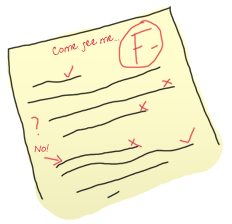
\includegraphics[width=1\linewidth]{exam.png}
\end{wrapfigure}
Логические ошибки искать и отлаживать сложнее всего. Чаще всего эти ошибки делает сам программист: ветвления и условия (например if\--ы и case\--ы), в которых не учитываются все случаи, употребление умножения вместо деления и т.д.
Такие ошибки не приводят к аварийному завершению программы, но из\--за них программа может просто выдать неверные данные или работать незапланированным образом.

С такими ошибками вам придётся справляться самостоятельно, но в Erlang есть много средств, которые придут вам на помощь.
В их числе тестовые фреймворки, TypEr и Dialyzer (которые описывались в \ref{for-type-junkies}~главе о типах), \ref{debugger-chapter}~отладчик, \ref{dbg}~модуль трассировки и т.д.
Лучшая защита от таких ошибок \--- это тестирование.
В карьере любого программиста, к сожалению, таких ошибок хватит на пару дюжин книг, поэтому я не буду тратить на них много времени.
Легче сконцентрироваться на тех ошибках, которые приводят к аварийному завершению, так как момент их появления ясен, и они не всплывут на поверхность через 50 уровней вложенности.
Это соображение, как раз, и служит источником мантры: <<пусть процесс падает>>, о которой я уже несколько раз упоминал.
\section{Ошибки времени исполнения}
\label{run-time-errors}
Ошибки времени исполнения (run\--time errors) весьма разрушительно влияют на ваш код. Они приводят к аварийной ситуации.
Хотя в Erlang и существуют методы их контроля, но никогда не бывает лишним умение эти ошибки различать.
Поэтому я составил небольшой список таких ошибок с объяснением и примерами кода, который может их вызвать.

\textbf{function\_clause}
\begin{lstlisting}[style=erlang]
1> lists:sort([3,2,1]).
[1,2,3]
2> lists:sort(fffffff).
** exception error: no function clause matching lists:sort(fffffff)
\end{lstlisting}

Все охранные выражения завершились неудачей, либо для функции не сработал ни один из шаблонов для сопоставления с образцом.
\blankline

\textbf{case\_clause}
\begin{lstlisting}[style=erlang]
3> case "Unexpected Value" of
3>    expected_value -> ok;
3>    other_expected_value -> 'also ok'
3> end.
** exception error: no case clause matching "Unexpected Value"
\end{lstlisting}

Похоже, что кто\--то забыл указать шаблон в выражении \ops{case}, передал неподходящие данные, или забыл задать вариант для выбора по умолчанию.
\blankline

\textbf{if\_clause}
\begin{lstlisting}[style=erlang]
4> if 2 > 4 -> ok;
4>    0 > 1 -> ok
4> end.
** exception error: no true branch found when evaluating an if expression
\end{lstlisting}

Это сообщение очень похоже на ошибки \ops{case\_clause}. Не получается найти ветку, которая принимает значение \ops{true}.
Скорее всего, необходимо убедиться, что обрабатываются все возможные случаи, либо добавить вариант \ops{true} для выбора по умолчанию.
\blankline

\textbf{badmatch}
\begin{lstlisting}[style=erlang]
5> [X,Y] = {4,5}.
** exception error: no match of right hand side value {4,5}
\end{lstlisting}

Такие ошибки возникают в случае, когда не удаётся провести операцию сопоставления с образцом.
Скорее всего, вы пытаетесь провести невозможное сопоставление, пытаетесь связать переменную со значением во второй раз, или по обе стороны оператора \ops{\strut=} находятся неравные значения (что, в общем\--то и приводит к тому, что операция связывания завершается неудачей!).
Заметьте, что иногда эта ошибка возникает, потому что по мнению программиста переменная вида \emph{\_MyVar} означает то же самое, что и \ops{\strut\_}.
Переменные, имя которых начинается со знака подчёркивания \--- это обычные переменные.
Единственное их отличие в том, что компилятор не генерирует предупреждение, если эти переменные не используются после объявления.
Их можно связать со значением лишь один раз.
\blankline

\textbf{badarg}
\begin{lstlisting}[style=erlang]
6> erlang:binary_to_list("heh, already a list").
** exception error: bad argument
    in function  binary_to_list/1
        called as binary_to_list("heh, already a list")
\end{lstlisting}

Эта ошибка похожа на \ops{function\_clause} тем, что она сообщает о вызове функции с некорректными аргументами.
Главное отличие в том, что ошибка генерируется программистом, который проверяет аргументы в теле функции, а не в охранных выражениях (стражах).
Чуть позже в этой главе я покажу как генерировать такие ошибки.
\blankline

\textbf{undef}
\begin{lstlisting}[style=erlang]
7> lists:random([1,2,3]).
** exception error: undefined function lists:random/1
\end{lstlisting}
Ошибка генерируется, когда вы пытаетесь вызвать несуществующую функцию.
Убедитесь, что функция экспортируется из модуля с правильной арностью (если вы вызываете её вне модуля), и перепроверьте правильность написания имени функции и модуля.
Ещё одной причиной получения этого сообщения может служить то, что модуль находится вне пути поиска Erlang.
По умолчанию поиск происходит в текущей директории. Добавлять пути можно при помощи функции \ops{code:add\_patha/1} или \ops{code:add\_pathz/1}.
Если ничего из перечисленного не помогает, то сперва убедитесь, что модуль скомпилирован!
\blankline

\textbf{badarith}
\begin{lstlisting}[style=erlang]
8> 5 + llama.
** exception error: bad argument in an arithmetic expression
    in operator  +/2
        called as 5 + llama
\end{lstlisting}

Это сообщение появляется, когда вы пытаетесь выполнить несуществующее арифметическое действие.
Например, делите на ноль или пытаетесь выполнять арифметические операции между атомами и числами.
\blankline

\textbf{badfun}
\begin{lstlisting}[style=erlang]
9> hhfuns:add(one,two).
** exception error: bad function one
in function  hhfuns:add/2
\end{lstlisting}
Чаще всего причиной возникновения этой ошибки становится попытка использовать переменные в качестве функций, но при этом переменные функций не содержат.
В приведённом выше примере я использую функцию \ops{hhfuns} из предыдущей главы \ref{higher-order-functions}~и при этом передаю в качестве параметров\--функций пару атомов.
Такой код не сработает, и будет выброшена ошибка \ops{badfun}.
\blankline

\textbf{badarity}
\begin{lstlisting}[style=erlang]
10> F = fun(_) -> ok end.
#Fun<erl_eval.6.13229925>
11> F(a,b).
** exception error: interpreted function with arity 1 called with two arguments
\end{lstlisting}
Ошибка \ops{badarity} \--- это частный случай ошибки \ops{badfun}. 
Она происходит, когда вы используете функции высшего порядка, которым передаёте больше (или меньше) аргументов, чем они требуют.
\blankline

\textbf{system\_limit}

Есть много причин, по которым может быть сгенерирована ошибка \ops{system\_limit}: слишком много процессов (мы до них ещё доберёмся), слишком длинные атомы, у функции слишком много аргументов, количество атомов слишком велико, слишком много подсоединённых узлов и т.д.
Полный список можно прочитать в \href{http://www.erlang.org/doc/efficiency_guide/advanced.html#id2265856}{Erlang Efficiency Guide} в разделе о системных ограничениях (system limits).
Примите к сведению, что некоторые из этих ошибок настолько серьёзны, что могут привести к аварии всей виртуальной машины.

\section{Вызываем исключения}
\label{raising-exceptions}
Чтобы следить за исполнением кода и защититься от логических ошибок, иногда полезно провоцировать аварийную остановку во время исполнения кода, чтобы как можно раньше выявить возможные проблемы.
В Erlang существуют три вида исключений: \emph{ошибки (errors)}, \emph{броски (throws)} и \emph{завершения (exits)}. Все они используются в разных случаях (ну или почти в разных):

\begin{wrapfigure}{r}{0.35\linewidth}
    
\includegraphics[width=1\linewidth]{stop.png}
\end{wrapfigure}

\subsection{Ошибки}
\label{errors}
Вызов \ops{erlang:error(Reason)} завершит исполнение в текущем процесе и, после того как исключение будет поймано, предоставит трассировку стека и список аргументов для последних вызовов функций.
Это тот самый вид исключений, который вызывает ошибки времени исполнения, о которых я упоминал выше.

При помощи ошибок (errors) можно останавливать исполнение, в случае когда вызываемый код не сможет сам справиться с создавшейся ситуацией.
Если вам была возвращена ошибка \ops{if\_clause}, что вы сделаете?
Измените код, перекомпилируете его \--- вот и всё что вы можете (ну, ещё можно отобразить красивое сообщение об ошибке).
Примером того, где не следует использовать ошибки, может служить наш модуль для работы с деревьями из главы о рекурсии \ref{recursion}.
Поиск по дереву, реализованный в модуле, не всегда в состоянии найти в дереве заданный ключ.
В такой ситуации имеет смысл ожидать, что с неизвестным результатом разберётся сам пользователь. 
Он сможет использовать значение по умолчанию, удалить дерево, вставить новое значение после проверки и т.д.
В этой ситуации вместо генерирования ошибки лучше было бы возвратить кортеж \ops{\{ok, Value\}}, или атом \ops{undefined}.

Но область применения ошибок не ограничивается лишь этими примерами.
Можно также определить собственный вид ошибок:
\begin{lstlisting}[style=erlang]
1> erlang:error(badarith).
** exception error: bad argument in an arithmetic expression
2> erlang:error(custom_error).
** exception error: custom_error
\end{lstlisting}

В этом примере оболочка Erlang не распознала \ops{custom\_error} и не вывела сообщение вида ``bad argument in \ldots'', но тем не менее эту ошибку можно использовать и обрабатывать так же как обычно (скоро мы увидим как это делать).

\subsection{Завершения}
\label{exits}
Существует два вида завершений: 'внутренние' (internal) и 'внешние' (external).
Внутренние завершения выполняются посредством вызова функции \ops{exit/1} и приводят к остановке текущего процесса.
Внешние завершения выполняются функцией \ops{exit/2} и имеют отношение к множеству процессов, принадлежащих к параллельной (concurrent) части Erlang; поэтому здесь мы сосредоточимся на внутренних завершениях, а к внешним обратимся чуть позже.

Внутренние завершения очень похожи на ошибки (errors).
На самом деле, раньше они никак не различались и существовала лишь одна функция \ops{exit/1}.
Использовали их в приблизительно одинаковых случаях.
Так как же определить, что использовать в конкретной ситуации?
Выбор неочевиден.
Чтобы понять, когда нужно использовать ту или иную конструкцию, ничего не остаётся кроме как начать издалека поглядывать на концепции акторов и процессов.

Во введении я сравнивал процессы с людьми, которые общаются посредством почты. К этой аналогии, в общем\--то, добавить нечего, поэтому перейду к диаграммам и кружкам.
\begin{figure}[h!]
    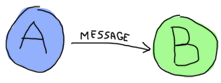
\includegraphics[width=0.4\textwidth]{a-b-msg.png}
\end{figure}

Процессы на этой картинке могут посылать друг другу сообщения.
Процесс также может ожидать прихода каких\--либо сообщений.
Можно выбирать, какие сообщения нужно ждать, какие отклонять, а какие игнорировать, через какой период времени прекращать ожидание и т.д.
\begin{figure}[h!]
    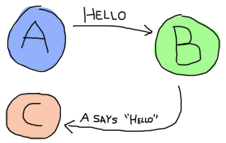
\includegraphics[width=0.4\textwidth]{a-b-c-hello.png}
\end{figure}

Эти основные концепции позволяют создателям Erlang использовать особенный вид сообщений, при помощи которых между процессами передаются исключения.
Они работают как своего рода <<последний вздох>> процесса; их посылают прямо перед тем, как процесс умирает, и его код перестаёт выполняться.
Другие процессы, которые ожидали этот вид сообщений, смогут узнать об этом событии и распорядиться этим знанием как угодно.
Сделать запись в журнале, перезапустить умерший процесс и т.д.
\begin{figure}[h!]
    
\includegraphics[width=0.4\textwidth]{a-b-dead.png}
\end{figure}

Ну а теперь, когда мы имеем представление об этой концепции, нам будет проще понять разницу между \ops{erlang:error/1} и \ops{exit/1}.
Обе функции можно использовать очень похожим способом, но настоящая разница заключается в нашем намерении.
После получения такой ошибки можно решить, была ли это <<просто>> ошибка или ошибка из\--за которой стоит убить текущий процесс.
Это соображение подкрепляется тем, что функция \ops{erlang:error/1} возвращает трассировку стека, а \ops{exit/1} этого не делает.
Если бы у текущей функции был длинный стек вызовов или много аргументов, то отсылка сообщений о её завершении каждому процессу, который их ожидает, означала бы, что эти данные пришлось бы копировать. В некоторых случаях это может стать непрактичным.
\subsection{Броски}
\label{throws}
Броски \--- это класс исключений, используемых в случаях, которые должен обрабатывать программист.
По сравнению с завершениями  или ошибками, броски не имеют коннотации <<роняй процесс!>>.
Они больше относятся к управлению логикой программы.
Так как вы используете броски в ожидании, что о них позаботится программист, то не лишним будет задокументировать этот факт в модуле, который их содержит.

Синтаксис бросков следующий:
\begin{lstlisting}[style=erlang]
1> throw(permission_denied).
** exception throw: permission_denied
\end{lstlisting}
\ops{permission\_denied} можно заменить чем угодно (даже сообщением \ops{'всё в порядке'}, но этим вы вряд ли кому-либо поможете, а вот друзей с таким кодом вы точно не приобретёте).

Броски также можно использовать для нелокального возврата из глубокой рекурсии.
Можно привести модуль \ops{\href{http://erldocs.com/R15B/ssl/ssl.html}{ssl}} в качестве примера.
Он использует функцию \ops{throw/1} для того, чтобы вернуть кортежи \ops{\{error, Reason\}} вызывающей функции.
А она, в свою очередь, просто возвращает кортеж пользователю.
Благодаря этому механизму разработчик может писать код, который рассматривает только благополучные варианты развития событий, а все исключения обрабатывает лишь в одной вышестоящей функции.

Ещё одним примером может послужить модуль для работы с массивами, в котором есть функция поиска.
В случае, если нужный элемент не был найден, эта функция возвращает значение по умолчанию, предоставленное пользователем.
Когда элемент не удаётся найти, в исключении бросается значение \ops{default}, которое обрабатывает вышестоящая функция и заменяет на пользовательское значение по умолчанию.
Это избавляет программиста модуля от необходимости передавать значение по умолчанию в каждую функцию алгоритма поиска и позволяет сконцентрироваться лишь на благополучных исходах.

Чтобы облегчить отладку кода, старайтесь сосредоточить все случаи использования бросков для нелокальных возвратов в одном модуле.
К тому же, это позволит изменять внутреннее устройство модуля без необходимости менять его интерфейс.
\section{Расправляемся с исключениями}
\label{dealing-with-exceptions}
Я уже много раз упоминал о том, что бросками, ошибками и завершениями можно управлять.
Для этого используют выражения \ops{try \ldots catch}.
\begin{wrapfigure}{r}{0.14\linewidth}
    
\includegraphics[width=1\linewidth]{catch.png}
\end{wrapfigure}
При помощи \ops{try \ldots catch} можно исполнить какое\--либо выражение, и обработать как случай успешного выполнения кода, так и возможные ошибки.
Для таких выражений используется следующий синтаксис:
\begin{lstlisting}[style=erlang]
try Expression of
    SuccessfulPattern1 [Guards] ->
        Expression1;
    SuccessfulPattern2 [Guards] ->
    Expression2
catch
    TypeOfError:ExceptionPattern1 ->
        Expression3;
    TypeOfError:ExceptionPattern2 ->
        Expression4
end.
\end{lstlisting}

О \emph{Выражении}, которое находится между \ops{try} и \ops{of} говорят, что оно \emph{защищено}. Это означает, что будет поймано любое исключение, вызванное этим выражением.
Шаблоны и выражения, которые используются в \ops{try \ldots of} и \ops{catch} ведут себя так же как и в \ops{case \ldots of}.
Также в \ops{catch} можно заменить \emph{TypeOfError} на \ops{error}, \ops{throw} либо \ops{exit}, для каждого соответcтвующего типа исключений, которые мы рассмотрели в этой главе.
Если не указывать тип исключения, то по умолчанию используется тип \ops{throw}.
Попробуем применить наши знания на практике.

Для начала создадим модуль под названием \ops{\href{http://learnyousomeerlang.com/static/erlang/exceptions.erl}{exceptions}}.
Ничего сложного выдумывать не будем:
\begin{lstlisting}[style=erlang]
-module(exceptions).
-compile(export_all).
 
throws(F) ->
    try F() of
        _ -> ok
    catch
        Throw -> {throw, caught, Throw}
    end.
\end{lstlisting}

Давайте скомпилируем модуль и опробуем его на разных видах исключений:
\begin{lstlisting}[style=erlang]
1> c(exceptions).
{ok,exceptions}
2> exceptions:throws(fun() -> throw(thrown) end).
{throw,caught,thrown}
3> exceptions:throws(fun() -> erlang:error(pang) end).
** exception error: pang
\end{lstlisting}

Как видите, \ops{try \ldots catch} принимает лишь броски (throws).
Как я и говорил ранее, без явного указания типа исключения используются броски.
А теперь запишем функции с catch для каждого типа:
\begin{lstlisting}[style=erlang]
errors(F) ->
    try F() of
        _ -> ok
    catch
        error:Error -> {error, caught, Error}
    end.
 
exits(F) ->
    try F() of
        _ -> ok
    catch
        exit:Exit -> {exit, caught, Exit}
    end.
\end{lstlisting}

И исполним их:
\begin{lstlisting}[style=erlang]
4> c(exceptions).
{ok,exceptions}
5> exceptions:errors(fun() -> erlang:error("Die!") end).
{error,caught,"Die!"}
6> exceptions:exits(fun() -> exit(goodbye) end).
{exit,caught,goodbye}
\end{lstlisting}

Следующий пример демонстрирует как комбинировать все виды исключений в одном \ops{try \ldots catch}.
Сначала объявим функцию, которая будет генерировать нужные нам исключения:
\begin{lstlisting}[style=erlang]
sword(1) -> throw(slice);
sword(2) -> erlang:error(cut_arm);
sword(3) -> exit(cut_leg);
sword(4) -> throw(punch);
sword(5) -> exit(cross_bridge).
 
black_knight(Attack) when is_function(Attack, 0) ->
    try Attack() of
        _ -> "None shall pass."
    catch
        throw:slice -> "It is but a scratch.";
        error:cut_arm -> "I've had worse.";
        exit:cut_leg -> "Come on you pansy!";
        _:_ -> "Just a flesh wound."
    end.
\end{lstlisting}

В этом примере используется встроенная функция \ops{is\_function/2}, при помощи которой проверяется, что переменная \emph{Attack} \--- это функция арности 0. А теперь добавим ещё одну:
\begin{lstlisting}[style=erlang]
talk() -> "blah blah".
\end{lstlisting}
\emph{А теперь кое\--что совершенно иное} (MP):
\begin{lstlisting}[style=erlang]
7> c(exceptions).
{ok,exceptions}
8> exceptions:talk().
"blah blah"
9> exceptions:black_knight(fun exceptions:talk/0).
"None shall pass."
10> exceptions:black_knight(fun() -> exceptions:sword(1) end).
"It is but a scratch."
11> exceptions:black_knight(fun() -> exceptions:sword(2) end).
"I've had worse."
12> exceptions:black_knight(fun() -> exceptions:sword(3) end).
"Come on you pansy!"
13> exceptions:black_knight(fun() -> exceptions:sword(4) end).
"Just a flesh wound."
14> exceptions:black_knight(fun() -> exceptions:sword(5) end).
"Just a flesh wound."
\end{lstlisting}

Выражение из 9\--й строки демонстрирует нормальное поведение чёрного рыцаря для случая, когда функция выполняется успешно.
В каждой последующей строчке показано сопоставление с образцом для исключений согласно их класса (бросок, ошибка, завершение), и причина их возникновения (\ops{slice}, \ops{cut\_arm}, \ops{cut\_leg}).

\begin{wrapfigure}{r}{0.35\linewidth}
    
\includegraphics[width=1\linewidth]{black-knight.png}
\end{wrapfigure}

В строках 13 и 14 показано выражение, которое используется для ловли исключений, когда все предыдущие выражния не сработали.
Шаблон \ops{\_:\_} используется в случае, когда вы хотите словить любое исключение какого угодно типа.
На практике следует использовать этот шаблон с осторожностью: старайтесь защитить ваш код от того, с чем можете справиться, но не более того.
Чтобы справиться со всем остальным, в Erlang есть другие средства.

После \ops{try \ldots catch} можно добавить дополнительное выражение, которое будет исполнено в любом случае.
Оно эквивалентно блоку 'finally', который используется во многих других языках:
\begin{lstlisting}[style=erlang]
try Expr of
    Pattern -> Expr1
catch
    Type:Exception -> Expr2
after % this always gets executed
    Expr3
end
\end{lstlisting}

Выражения внутри \ops{after} будут гарантированно исполнены независимо от того, возникли ошибки или нет.
Стоит отметить, что конструкция \ops{after} не возвращает результат.
Поэтому её можно использовать лишь для исполнения кода с побочными эффектами.
Каноническим примером использования этой конструкции может служит ситуация, когда вы хотите убедиться, что файл, из которого вы читаете данные, будет закрыт независимо от того, возникали исключения или нет.

Теперь мы знаем как управлять в Erlang тремя классами исключений при помощи блоков catch.
Но я кое о чём умолчал!
Между \ops{try} и {of} можно поместить не одно выражение, а несколько!
\begin{lstlisting}[style=erlang]
whoa() ->
    try
        talk(),
        _Knight = "None shall Pass!",
        _Doubles = [N*2 || N <- lists:seq(1,100)],
        throw(up),
        _WillReturnThis = tequila
    of
        tequila -> "hey this worked!"
    catch
        Exception:Reason -> {caught, Exception, Reason}
    end.
\end{lstlisting}

При вызове \ops{exceptions:whoa()} мы явно получим \ops{\{caught, throw, up\}} из\--за \ops{throw(up)}.
Так что да, между \ops{try} и \ops{of} можно помещать несколько выражений\ldots

В \ops{exceptions:whoa/0} я попытался показать (а вы, вероятно этого не заметили), что когда мы используем много выражений, нам не всегда важен возвращаемый результат.
Поэтому часть \ops{of} становится чуть\--чуть бесполезной.
Ну и прекрасно, ведь её можно просто убрать:
\begin{lstlisting}[style=erlang]
im_impressed() ->
    try
        talk(),
        _Knight = "None shall Pass!",
        _Doubles = [N*2 || N <- lists:seq(1,100)],
        throw(up),
        _WillReturnThis = tequila
    catch
        Exception:Reason -> {caught, Exception, Reason}
    end.
\end{lstlisting}

Так\--то лучше!

\colorbox{lgray}
{
\begin{minipage}{1.0\linewidth}
    \textbf{Замечание:} важно понимать, что защищённая от исключений часть кода не может использовать хвостовую рекурсию.
    Виртуальная машина должна постоянно держать ссылку на этот код, на случай если возникнет исключение.

    Так как в конструкции \ops{try \ldots catch} без части \ops{of} нет ничего кроме защищённой части, то вызов рекурсивной функции из этой области кода может быть небезопасным для программы, которая должна находиться в запущенном состоянии долгое время (такие программы, как раз \--- ниша Erlang).
    Через определённое количество итераций на вашей машине закончится память, или ваша программа начнёт замедлятся без явных на то причин.
    Если вы поместите рекурсивные вызовы между \ops{of} и \ops{catch}, то они будут происходить вне защищённой части, и для них будет выполняться оптимизация последнего вызова.

    Некоторые люди  используют по умолчанию \ops{try \ldots of \ldots catch} вместо \ops{try \ldots catch}, чтобы избежать неожиданных ошибок такого типа.
    Такая осторожность излишня лишь в коде, который явно не содержит рекурсивные вызовы, и результаты выполнения которого не будут больше нигде использованы. Ну, вы и сами наверняка можете решить, как поступать в такой ситуации!
\end{minipage}
}
\section{Но это ещё не всё!}
\label{wait-theres-more}
Казалось бы, этих средств и так достаточно, чтобы быть наравне с другими языками программирования, но в Erlang есть ещё одна структура для управления ошибками.
Эта структура определяется ключевым словом \ops{catch} и, по сути, вдобавок к верным результатам может возвращать все типы исключений.
Она может показаться несколько странной, так как отображает исключения немного иначе:
\begin{lstlisting}[style=erlang]
1> catch throw(whoa).
whoa
2> catch exit(die).
{'EXIT',die}
3> catch 1/0.
{'EXIT',{badarith,[{erlang,'/',[1,0]},
            {erl_eval,do_apply,5},
            {erl_eval,expr,5},
            {shell,exprs,6},
            {shell,eval_exprs,6},
{shell,eval_loop,3}]}}
4> catch 2+2.
4
\end{lstlisting}

В этом примере мы видим, что отображение бросков осталось прежним, а завершения и ошибки представлены в виде кортежей \ops{\{'EXIT', Reason\}}.
Это вызвано тем, что ошибки были вмонтированы в язык после завершений (для них оставили схожее представление для обратной совместимости).

Вот как следует читать эту трассировку стека:
\begin{lstlisting}[style=erlang]
5> catch doesnt:exist(a,4).             
{'EXIT',{undef,[{doesnt,exist,[a,4]},
            {erl_eval,do_apply,5},
            {erl_eval,expr,5},
            {shell,exprs,6},
            {shell,eval_exprs,6},
{shell,eval_loop,3}]}}
\end{lstlisting}
\begin{itemize}
    \item Тип этой ошибки \--- \ops{undef}. Это означает, что вызванная функция не определена (см. список в начале главы).
    \item Сразу за типом ошибки следует трассировка стека.
    \item Кортеж в самом начале трассировки обозначает последнюю функцию, которая должна была быть вызвана (\ops{\{Module, Function, Arguments\}}).
        Это та самая неопределённая функция.
    \item Кортежи, следующие за первым \--- это функции, которые вызывались перед тем как произошла ошибка.
        Здесь они принимают форму кортежа \ops{\{Module, Function, Arity\}}.
    \item В общем\--то, вот и всё.
\end{itemize}

Также можно вручную получить трассировку стека, вызывая функцию \ops{erlang:get\_stacktrace/0} внутри аварийного процесса.

Часто можно увидеть \ops{catch}, записанную следующим образом (мы всё ещё рассматриваем \href{http://learnyousomeerlang.com/static/erlang/exceptions.erl}{exceptions.erl}):
\begin{lstlisting}[style=erlang]
catcher(X,Y) ->
    case catch X/Y of
        {'EXIT', {badarith,_}} -> "uh oh";
        N -> N
    end.
\end{lstlisting}

И, как мы и ожидали:
\begin{lstlisting}[style=erlang]
6> c(exceptions).
{ok,exceptions}
7> exceptions:catcher(3,3).
1.0
8> exceptions:catcher(6,3).
2.0
9> exceptions:catcher(6,0).
"uh oh"
\end{lstlisting}

На первый взгляд этот способ перехвата исключений выглядит компактным и простым, но у \ops{catch} есть несколько особенностей.
Первая \--- это порядок выполнения операций:
\begin{lstlisting}[style=erlang]
10> X = catch 4+2.
* 1: syntax error before: 'catch'
10> X = (catch 4+2).
6
\end{lstlisting}

То, что в примере необходимы скобки, не вполне согласуется с интуицией, если учесть, что большинство выражений в скобки заключать не нужно.
Ещё одна проблема заключается в том, что невозможно отличить представление исключения от настоящего исключения:
\begin{lstlisting}[style=erlang]
11> catch erlang:boat().
{'EXIT',{undef,[{erlang,boat,[]},
            {erl_eval,do_apply,5},
            {erl_eval,expr,5},
            {shell,exprs,6},
            {shell,eval_exprs,6},
{shell,eval_loop,3}]}}
12> catch exit({undef, [{erlang,boat,[]}, {erl_eval,do_apply,5}, {erl_eval,expr,5}, {shell,exprs,6}, {shell,eval_exprs,6}, {shell,eval_loop,3}]}).
{'EXIT',{undef,[{erlang,boat,[]},
            {erl_eval,do_apply,5},
            {erl_eval,expr,5},
            {shell,exprs,6},
            {shell,eval_exprs,6},
{shell,eval_loop,3}]}}
\end{lstlisting}

И ошибку невозможно отличить от, собственно, самого завершения.
Чтобы сгенерировать исключение, приведённое выше, можно было бы также использовать функцию \ops{throw/1}.
Надо сказать, что использование \ops{throw/1} в \ops{catch} может также представлять собой проблему в другом контексте:
\begin{lstlisting}[style=erlang]
one_or_two(1) -> return;
one_or_two(2) -> throw(return).
\end{lstlisting}

А вот и страшная проблема:
\begin{lstlisting}[style=erlang]
13> c(exceptions).
{ok,exceptions}
14> catch exceptions:one_or_two(1).
return
15> catch exceptions:one_or_two(2).
return
\end{lstlisting}

Так как мы находимся за \ops{catch}, то никогда не знаем наверняка, бросила ли функция исключение или вернула результат!
На практике это случается не очень часто, но эта особенность повлекла за собой появление конструкции \ops{try \ldots catch} в релизе R10B.
